\documentclass{ctexart}
\usepackage{amsmath, amsfonts, amssymb} % 数学公式、符号
\usepackage[colorlinks,linkcolor=red,anchorcolor=blue,citecolor=green]{hyperref}
\usepackage[left=2.10cm, right=2.10cm, top=1.50cm, bottom=1.50cm]{geometry} %页边距
\usepackage{graphicx}   % 图片
\usepackage{multicol}
\usepackage{bm}
\usepackage{listings}
\usepackage{xcolor}
\usepackage{tikz}
\usetikzlibrary{arrows,shapes,chains}
\usepackage{multirow}
\usepackage{algorithm}  
\usepackage{algpseudocode}  
\usepackage{caption}
\floatname{algorithm}{算法}
\renewcommand{\algorithmicrequire}{\textbf{输入:}}  % Use Input in the format of Algorithm  
\renewcommand{\algorithmicensure}{\textbf{输出:}} % Use Output in the format of Algorithm
\usepackage{fancyhdr} %设置页眉、页脚
\pagestyle{fancy}
% 用来设置代码的样式
\lstset{
	basicstyle          =   \sffamily,          % 基本代码风格
	keywordstyle        =   \bfseries,          % 关键字风格
	commentstyle        =   \rmfamily\itshape,  % 注释的风格,斜体
	stringstyle         =   \ttfamily,  % 字符串风格
	flexiblecolumns,                % 别问为什么,加上这个
	numbers             =   left,   % 行号的位置在左边
	showspaces          =   false,  % 是否显示空格,显示了有点乱,所以不现实了
	numberstyle         =   \zihao{-5}\ttfamily,    % 行号的样式,小五号,tt等宽字体
	showstringspaces    =   false,
	captionpos          =   t,      % 这段代码的名字所呈现的位置,t指的是top上面
	frame               =   lrtb,   % 显示边框
}

\lstdefinestyle{Python}{
	language        =   Python, % 语言选Python
	basicstyle      =   \zihao{-5}\ttfamily,
	numberstyle     =   \zihao{-5}\ttfamily,
	keywordstyle    =   \color{blue},
	keywordstyle    =   [2] \color{teal},
	stringstyle     =   \color{magenta},
	commentstyle    =   \color{red}\ttfamily,
	breaklines      =   true,   % 自动换行,建议不要写太长的行
	columns         =   fixed,  % 如果不加这一句,字间距就不固定,很丑,必须加
	basewidth       =   0.5em,
}

\title{\textbf{机器学习实验报告\\{\Large{支持向量机}}}} % 标题与子标题
\author{\sffamily{朱天泽}} % 作者
\date{(日期:\today)} % 日期
\vspace{0.7cm}
\setlength{\abovecaptionskip}{0.3cm}   %调整图片标题与图距离
\captionsetup{font={small}}
\setlength{\belowcaptionskip}{0.1cm}   %调整图片标题与下文距离
\begin{document}
	\maketitle
	% 摘要开始
	\noindent{\bf{摘要}}
	在《机器学习》第6章中,我学习了支持向量机。此次实验,我实现了使用核函数和软间隔的支持向量机,在西瓜数据集$3.0\alpha$上用多个核函数进行了训练,并对不同核函数的分类效果进行了比较。
	
	\noindent{\bf{关键词}} SVM;核函数;分类
	
	% 正文开始
	\section{题目理解}
	题目要求:在西瓜数据集 $3.0\alpha$ 上分别用线性核和高斯核训练一个SVM。
	
	针对不同的核函数 $\kappa$,其底层的数学原理都类似,给一个SVM替换核函数也相对方便。因此本次实验计划不止用线性核和高斯核训练SVM,而是使用多个核函数分别训练一个SVM,并对不同核函数得到的SVM的分类效果做对比。
	\section{支持向量机原理阐述}
	\subsection{间隔与支持向量}
	给定训练样本集 $D=\{(\bm{x}_1,y_1),(\bm{x}_2,y_2),\cdots,(\bm{x}_m,y_m)\}$,$y_i\in\{-1,1\}$,分类学习最基本的想法是基于训练集$D$在样本空间中找到一个划分超平面,将不同类别的样本分开。
	
	在样本空间中,划分超平面可通过如下线性方程来描述:
	
	\begin{equation}
		\boldsymbol{w}^{\mathrm{T}} \boldsymbol{x}+b=0
	\end{equation}

	其中 $\boldsymbol{w}=(w_1,w_2,\cdots,w_d)^{\mathrm{T}}$ 为超平面的法向量,$b$ 为位移项,决定了超平面与原点之间的距离。显然,划分超平面可被法向量 $\boldsymbol{w}$ 和位移$b$确定,下面我们将超平面记为 $(\boldsymbol{w},b)$。
	
	对于任意一点 $\boldsymbol{x}_{0}=\left(x_{1}^{0}, x_{2}^{0}, \cdots, x_{n}^{0}\right)^{\mathrm{T}}$, 设其在超平面 $\boldsymbol{w}^{\mathrm{T}} \boldsymbol{x}+b=0$ 上的投影点为 $\boldsymbol{x}_{1}=\left(x_{1}^{1}, x_{2}^{1}, \cdots, x_{n}^{1}\right)^{\mathrm{T}}$, 则 $\boldsymbol{w}^{\mathrm{T}} \boldsymbol{x}_{1}+b=0$, 设其到超平面的距离为 $r$;由于向量 $\overrightarrow{\boldsymbol{x}_{1} \boldsymbol{x}_{0}}$ 与法向量 $\boldsymbol{w}$ 平行,因此
	
	\begin{equation}
		\left|\boldsymbol{w} \cdot \overrightarrow{\boldsymbol{x}_{1} \boldsymbol{x}_{0}}\right|=\left|\|\boldsymbol{w}\| \cdot \cos \pi \cdot\left\|\overrightarrow{\boldsymbol{x}_{1} \boldsymbol{x}_{0}}\right\|\right|=\|\boldsymbol{w}\| \cdot\left\|\overrightarrow{\boldsymbol{x}_{1} \boldsymbol{x}_{0}}\right\|=\|\boldsymbol{w}\| \cdot r 
	\end{equation}
	
	又有
	\begin{equation}
		\begin{aligned}
			\boldsymbol{w} \cdot \overrightarrow{\boldsymbol{x}_{1} \boldsymbol{x}_{0}} &=w_{1}\left(x_{1}^{0}-x_{1}^{1}\right)+w_{2}\left(x_{2}^{0}-x_{2}^{1}\right)+\cdots+w_{n}\left(x_{n}^{0}-x_{n}^{1}\right) \\
			&=w_{1} x_{1}^{0}+w_{2} x_{2}^{0}+\cdots+w_{n} x_{n}^{0}-\left(w_{1} x_{1}^{1}+w_{2} x_{2}^{1}+\cdots+w_{n} x_{n}^{1}\right) \\
			&=\boldsymbol{w}^{\mathrm{T}} \boldsymbol{x}_{0}-\boldsymbol{w}^{\mathrm{T}} \boldsymbol{x}_{1} \\
			&=\boldsymbol{w}^{\mathrm{T}} \boldsymbol{x}_{0}+b
		\end{aligned}
	\end{equation}
	
	故 $\left|\boldsymbol{w}^{\mathrm{T}} \boldsymbol{x}_{0}+b\right|=\|\boldsymbol{w}\| \cdot r$,因此对于任意点 $\boldsymbol{x}$,其到超平面 $(\boldsymbol{w},b)$ 的距离为
	
	\begin{equation}
		r=\frac{\left|\boldsymbol{w}^{\mathrm{T}} \boldsymbol{x}+b\right|}{\|\boldsymbol{w}\|}
	\end{equation}

	将训练样本分开的划分超平面有很多,如图\ref{正中间}。直观上看应该去找位于两类训练样本“正中间”的划分超平面,即距离超平面最近的正反例到超平面的距离“相当”,该划分超平面对训练样本局部扰动的容忍性最好。例
	如,由于训练集的局限性或噪声的因素,训练集外的样本可能比图\ref{正中间}中的训练
	样本更接近两个类的分隔界,这将使许多划分超平面出现错误,而“正中间”的超平
	面受影响最小。换言之,这个划分超平面所产生的分类结果是最鲁棒的,对未见
	示例的泛化能力最强。
	
	\begin{figure}[!htb]
		\centering
		\begin{minipage}{0.49\linewidth}
			\centering
			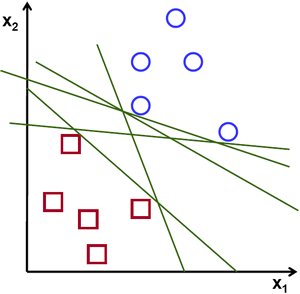
\includegraphics[width=0.6\textwidth]{../image/正中间.png}
		\end{minipage}
		\begin{minipage}{0.49\linewidth}
			\centering
			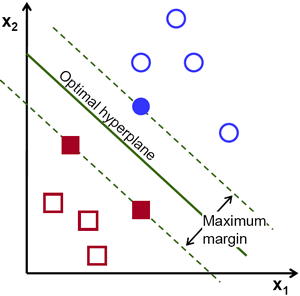
\includegraphics[width=0.6\textwidth]{../image/正中间y.png}
		\end{minipage}
		\caption{有多个划分超平面将两类训练样本分开}
		\label{正中间}
	\end{figure}
	
	对于给定的数据集 $D$ 和超平面 $(\boldsymbol{w},b)$,定义任意一个样本点 $(\boldsymbol{x}_i,y_i)$,$y_i\in\{-1,1\}$,$i=1,2,\cdots,m$ 关于超平面的几何间隔为
	
	\begin{equation}
		\gamma_{i}=\frac{y_{i}\left(\boldsymbol{w}^{\mathrm{T}} \boldsymbol{x}_{i}+b\right)}{\|\boldsymbol{w}\|}
	\end{equation}

	当对样本 $(\boldsymbol{x}_i,y_i)$正确分类时,$\gamma_{i}>0$,几何间隔此时也等价于点到超平面的距离;而没有正确分类时,$\gamma_{i}<0$。
	
	对于给定的数据集 $D$ 和超平面 $(\boldsymbol{w},b)$,定义数据集 $D$ 关于超平面的几何间隔为数据集 $D$ 中所有样本点的几何间隔最小值
	
	\begin{equation}
		\gamma=\min _{i=1,2, \cdots, m} \gamma_{i}
	\end{equation}
	
	给定线性可分数据集 $D$,支持向量机模型希望求得使得数据集 $D$ 的几何间隔 $\gamma$ 达到最大的超平面,然后利用 $\operatorname{sign}$ 函数实现分类功能
	
	\begin{equation}
		y=\operatorname{sign}\left(\boldsymbol{w}^{\mathrm{T}} \boldsymbol{x}+b\right)=\left\{\begin{aligned}
			1, & \boldsymbol{w}^{\mathrm{T}} \boldsymbol{x}+b>0 \\
			-1, & \boldsymbol{w}^{\mathrm{T}} \boldsymbol{x}+b<0
		\end{aligned}\right.
	\end{equation}

	易知:
	
	\begin{itemize}
		\item 当超平面没有正确划分样本时,必存在 $\gamma_{i}<0$,故 $\gamma<0$;
		\item 当超平面正确划分样本时,有 $\gamma\geqslant 0$,且越靠近样本间隔中央 $\gamma$ 越大
	\end{itemize}

	因此,使得几何间隔 $\gamma$ 最大的超平面就是位于两类训练样本“正中间”的划分超平面。
	
	给定线性可分数据集 $D$,设 $D$ 中几何间隔最小的样本为 $(\boldsymbol{x}_\text{min},y_\text{min})$,称其为“支持向量”,如图\ref{支持向量}所示。
	
	\begin{figure}[!htb]
		\centering
		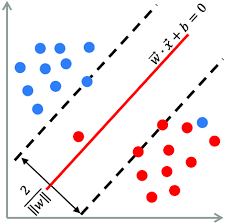
\includegraphics[width=0.3\textwidth]{../image/支持向量与几何间隔.png}
		\caption{支持向量与几何间隔}
		\label{支持向量}
	\end{figure}
	
	SVM寻找最优超平面的过程可以转化为如下带约束条件的优化问题
	
	\begin{equation}
		\begin{aligned}
			&\max\quad \gamma\\
			&\ \text{s.t.} \quad \gamma_{i} \geqslant \gamma, \quad i=1,2, \cdots, m
		\end{aligned}
	\end{equation}

	即
	
	\begin{equation}
		\begin{aligned}
			\max _{\boldsymbol{w}, b} & \frac{y_{\min }\left(\boldsymbol{w}^{\mathrm{T}} \boldsymbol{x}_{\min }+b\right)}{\|\boldsymbol{w}\|} \\
			\text { s.t. } & y_{i}\left(\boldsymbol{w}^{\mathrm{T}} \boldsymbol{x}_{i}+b\right) \geqslant y_{\min }\left(\boldsymbol{w}^{\mathrm{T}} \boldsymbol{x}_{\min }+b\right), \quad i=1,2, \cdots, m
		\end{aligned}
	\end{equation}

	假设该问题的最优解为 $(\boldsymbol{w}^\ast,b^\ast)$,那么 $(k\boldsymbol{w}^\ast,kb^\ast)$,$k\in\mathbb{R}^+$ 也是最优解,且超平面不变,因此需要对 $(\boldsymbol{w},b)$ 做一定限制才能使得上述优化问题有唯一解。那么不妨令 $y_{\min }\left(\boldsymbol{w}^{\mathrm{T}} \boldsymbol{x}_{\min }+b\right)=1$,对于特定的 $(\boldsymbol{x}_{\min},y_{\min})$ 来说,能使得 $y_{\min }\left(\boldsymbol{w}^{\mathrm{T}} \boldsymbol{x}_{\min }+b\right)=1$ 的 $k$ 有且仅有一个。因此,上述优化问题进一步转化为
	
	\begin{equation}
		\begin{array}{ll}
			\max\limits_{\boldsymbol{w}, b} & \frac{1}{\|\boldsymbol{w}\|} \\
			\text { s.t. } & y_{i}\left(\boldsymbol{w}^{\mathrm{T}} \boldsymbol{x}_{i} +b\right) \geqslant 1, \quad i=1,2, \cdots, m
		\end{array}
	\end{equation}

	上述问题等价于
	
	\begin{equation}
		\begin{array}{ll}
			\min\limits_{w, b} & \frac{1}{2}\|\boldsymbol{w}\|^{2} \\
			\text { s.t. } & 1-y_{i}\left(\boldsymbol{w}^{\mathrm{T}} \boldsymbol{x}_{i}+b\right) \leqslant 0, \quad i=1,2, \cdots, m
		\end{array}
		\label{主问题}
	\end{equation}

	这就是SVM的基本型。
	
	\subsection{对偶问题}
	
	我们称式\eqref{主问题}为主问题,对式\eqref{主问题}使用拉格朗日乘子法,其拉格朗日函数为
	
	\begin{equation}
		L(\boldsymbol{w}, b, \boldsymbol{\alpha})=\frac{1}{2}\|\boldsymbol{w}\|^{2}+\sum_{i=1}^{m} \alpha_{i}\left(1-y_{i}\left(\boldsymbol{w}^{\mathrm{T}} \boldsymbol{x}_{i}+b\right)\right)
		\label{拉格朗日函数}
	\end{equation}

	其中 $\boldsymbol{\alpha}=(\alpha_{1},\alpha_{2},\cdots,\alpha_{m})^\mathrm{T}$。令 $L(\boldsymbol{w}, b, \boldsymbol{\alpha})$ 对 $\boldsymbol{w}$ 和 $b$ 的偏导数都为零,可得
	
	\begin{equation}
		\boldsymbol{w}=\sum_{i=1}^{m} \alpha_{i} y_{i} \boldsymbol{x}_{i}
		\label{w约束}
	\end{equation}
	
	\begin{equation}
		\sum_{i=1}^{m} \alpha_{i} y_{i}=0
		\label{b约束}
	\end{equation}

	将式\eqref{w约束}代入\eqref{拉格朗日函数}
	
	\begin{equation}
		\begin{aligned}
			\inf _{\boldsymbol{w}, b} L(\boldsymbol{w}, b, \boldsymbol{\alpha}) &=\frac{1}{2} \boldsymbol{w}^{T} \boldsymbol{w}+\sum_{i=1}^{m} \alpha_{i}-\sum_{i=1}^{m} \alpha_{i} y_{i} \boldsymbol{w}^{T} \boldsymbol{x}_{i}-\sum_{i=1}^{m} \alpha_{i} y_{i} b \\
			&=\frac{1}{2} \boldsymbol{w}^{T} \sum_{i=1}^{m} \alpha_{i} y_{i} \boldsymbol{x}_{i}-\boldsymbol{w}^{T} \sum_{i=1}^{m} \alpha_{i} y_{i} \boldsymbol{x}_{i}+\sum_{i=1}^{m} \alpha_{i}-b \sum_{i=1}^{m} \alpha_{i} y_{i} \\
			&=-\frac{1}{2} \boldsymbol{w}^{T} \sum_{i=1}^{m} \alpha_{i} y_{i} \boldsymbol{x}_{i}+\sum_{i=1}^{m} \alpha_{i}-b \sum_{i=1}^{m} \alpha_{i} y_{i}
		\end{aligned}
		\label{对偶问题中间形态}
	\end{equation}

	再将\eqref{b约束}代入\eqref{对偶问题中间形态},于是有
	
	\begin{equation}
		\begin{aligned}
			\inf _{\boldsymbol{w}, b} L(\boldsymbol{w}, b, \boldsymbol{\alpha}) &=-\frac{1}{2} \boldsymbol{w}^{T} \sum_{i=1}^{m} \alpha_{i} y_{i} \boldsymbol{x}_{i}+\sum_{i=1}^{m} \alpha_{i} \\
			&=-\frac{1}{2}\left(\sum_{i=1}^{m} \alpha_{i} y_{i} \boldsymbol{x}_{i}\right)^{T}\left(\sum_{i=1}^{m} \alpha_{i} y_{i} \boldsymbol{x}_{i}\right)+\sum_{i=1}^{m} \alpha_{i} \\
			&=-\frac{1}{2} \sum_{i=1}^{m} \alpha_{i} y_{i} \boldsymbol{x}_{i}^{T} \sum_{i=1}^{m} \alpha_{i} y_{i} \boldsymbol{x}_{i}+\sum_{i=1}^{m} \alpha_{i} \\
			&=\sum_{i=1}^{m} \alpha_{i}-\frac{1}{2} \sum_{i=1}^{m} \sum_{j=1}^{m} \alpha_{i} \alpha_{j} y_{i} y_{j} \boldsymbol{x}_{i}^{T} \boldsymbol{x}_{j}
		\end{aligned}
	\end{equation}
	
	最终得到式\eqref{主问题}的对偶问题
	
	\begin{equation}
		\begin{aligned}
			&\max _{\boldsymbol{\alpha}} \sum_{i=1}^{m} \alpha_{i}-\frac{1}{2} \sum_{i=1}^{m} \sum_{j=1}^{m} \alpha_{i} \alpha_{j} y_{i} y_{j} \boldsymbol{x}_{i}^{\mathrm{T}}\boldsymbol{x}_j \\
			&\text { s.t. } \quad \sum_{i=1}^{m} \alpha_{i} y_{i}=0 \\
			&\ \quad\quad\quad \alpha_{i} \geqslant 0, \quad i=1,2, \cdots, m
		\end{aligned}
	\end{equation}

	注意到主问题,即式\eqref{主问题},是凸优化问题,且除支持向量外,存在样本点满足 $1-y_i(\boldsymbol{w}^{\mathrm{T}}\boldsymbol{x}_i+b)<0$;因此强对偶性成立,对偶问题的解就是原问题的解,且必须满足KKT条件
	
	\begin{equation}
		\left\{\begin{array}{l}
			\alpha_{i} \geqslant 0 \\
			y_{i} f\left(\boldsymbol{x}_{i}\right)-1 \geqslant 0 \\
			\alpha_{i}\left(y_{i} f\left(\boldsymbol{x}_{i}\right)-1\right)=0
		\end{array}\right.
		\label{KKT}
	\end{equation}

	解得 $\boldsymbol{\alpha}$ 后,求出 $\boldsymbol{w}$ 和 $b$ 即可得到模型
	
	\begin{equation}
		\begin{aligned}
			f(\boldsymbol{x}) &=\boldsymbol{w}^{\mathrm{T}} \boldsymbol{x}+b \\
			&=\sum_{i=1}^{m} \alpha_{i} y_{i} \boldsymbol{x}_{i}^{\mathrm{T}} \boldsymbol{x}+b
		\end{aligned}
	\end{equation}
	
		\subsection{核函数}
	
	在前面的讨论中,我们假设训练样本是线性可分的,即存在一个划分
	超平面能将训练样本正确分类。然而在现实任务中,原始样本空间内也许并不
	存在一个能正确划分两类样本的超平面。对这样的问题,可将样本从原始空间映射到-个更高维的特征空间,使得
	样本在这个特征空间内线性可分。
	
	令 $\phi(\boldsymbol{x})$ 表示将 $\boldsymbol{x}$ 映射后的特征向量,于是,在特征空间中划分超平面所对应的模型可表示为
	
	\begin{equation}
		f(x)=w^{\mathrm{T}} \phi(x)+b
	\end{equation}
	
	其中 $\boldsymbol{w}$ 和 $b$ 是模型参数。类似式\eqref{主问题},有
	
	\begin{equation}
		\begin{array}{ll}
			\min\limits_{\boldsymbol{w}, b} & \frac{1}{2}\|\boldsymbol{w}\|^{2} \\
			\text { s.t. } &1- y_{i}\left(\boldsymbol{w}^{\mathrm{T}} \phi\left(\boldsymbol{x}_{i}\right)+b\right) \leqslant 0, \quad i=1,2, \cdots, m
		\end{array}
	\end{equation}
	
	其对偶问题是 
	
	\begin{equation}
		\begin{aligned}
			&\max _{\boldsymbol{\alpha}} \sum_{i=1}^{m} \alpha_{i}-\frac{1}{2} \sum_{i=1}^{m} \sum_{j=1}^{m} \alpha_{i} \alpha_{j} y_{i} y_{j} \phi(\boldsymbol{x}_{i})^{\mathrm{T}}\phi(\boldsymbol{x}_j) \\
			&\text { s.t. } \quad \sum_{i=1}^{m} \alpha_{i} y_{i}=0 \\
			&\ \quad\quad\quad \alpha_{i} \geqslant 0, \quad i=1,2, \cdots, m
		\end{aligned}
		\label{带映射的原问题}
	\end{equation}
	
	求解式\eqref{带映射的原问题}涉及到计算 $\phi\left(\boldsymbol{x}_{i}\right)^{\mathrm{T}} \phi\left(\boldsymbol{x}_{j}\right)$,这是样本 $\boldsymbol{x}_i$ 与 $\boldsymbol{x}_j$ 映射到特征空间之后的内积。由于特征空间维数可能很高,甚至可能是无穷维,因此直接计算 $\phi\left(\boldsymbol{x}_{i}\right)^{\mathrm{T}} \phi\left(\boldsymbol{x}_{j}\right)$ 通常是困难的。为了避免这样的障碍,可以使用核技巧,定义核函数
	\begin{equation}
		\kappa\left(\boldsymbol{x}_{i}, \boldsymbol{x}_{j}\right)=\left\langle\phi\left(\boldsymbol{x}_{i}\right), \phi\left(\boldsymbol{x}_{j}\right)\right\rangle=\phi\left(\boldsymbol{x}_{i}\right)^{\mathrm{T}} \phi\left(\boldsymbol{x}_{j}\right)
	\end{equation}
	即 $\boldsymbol{x}_i$ 与 $\boldsymbol{x}_j$ 在特征空间中的内积等于它们在原始样本空间中通过函数 $\kappa(\cdot,\cdot)$ 计算的结果。有了核函数,我们就不必直接去计算高维甚至无穷维特征空间中的内积,于是式\eqref{带映射的原问题}可重写为
	
	\begin{equation}
		\begin{aligned}
			\max _{\boldsymbol{\alpha}} & \sum_{i=1}^{m} \alpha_{i}-\frac{1}{2} \sum_{i=1}^{m} \sum_{j=1}^{m} \alpha_{i} \alpha_{j} y_{i} y_{j} \kappa\left(\boldsymbol{x}_{i}, \boldsymbol{x}_{j}\right) \\
			\text { s.t. } & \sum_{i=1}^{m} \alpha_{i} y_{i}=0, \\
			& \alpha_{i} \geqslant 0, \quad i=1,2, \ldots, m
		\end{aligned}
	\end{equation}
	
	求解后即可得到
	
	\begin{equation}
		\begin{aligned}
			f(\boldsymbol{x}) &=\boldsymbol{w}^{\mathrm{T}} \phi(\boldsymbol{x})+b \\
			&=\sum_{i=1}^{m} \alpha_{i} y_{i} \phi\left(\boldsymbol{x}_{i}\right)^{\mathrm{T}} \phi(\boldsymbol{x})+b \\
			&=\sum_{i=1}^{m} \alpha_{i} y_{i} \kappa\left(\boldsymbol{x}, \boldsymbol{x}_{i}\right)+b
		\end{aligned}
		\label{fx}
	\end{equation}

	\textbf{定理}\ \ 令 $\chi$ 为输入空间,$\kappa(\cdot,\cdot)$是定义在 $\chi\times\chi$ 上的对称核函数,则 $\kappa$ 是核函数当且仅当对于任意数据 $D={\boldsymbol{x}_i}_{i=1}^m$,“核矩阵”$\mathbf{K}$ 总是半正定的:
	
	\begin{center}
		$\mathbf{K}=\left[\begin{array}{ccccc}
			\kappa\left(\boldsymbol{x}_{1}, \boldsymbol{x}_{1}\right) & \cdots & \kappa\left(\boldsymbol{x}_{1}, \boldsymbol{x}_{j}\right) & \cdots & \kappa\left(\boldsymbol{x}_{1}, \boldsymbol{x}_{m}\right) \\
			\vdots & \ddots & \vdots & \ddots & \vdots \\
			\kappa\left(\boldsymbol{x}_{i}, \boldsymbol{x}_{1}\right) & \cdots & \kappa\left(\boldsymbol{x}_{i}, \boldsymbol{x}_{j}\right) & \cdots & \kappa\left(\boldsymbol{x}_{i}, \boldsymbol{x}_{m}\right) \\
			\vdots & \ddots & \vdots & \ddots & \vdots \\
			\kappa\left(\boldsymbol{x}_{m}, \boldsymbol{x}_{1}\right) & \cdots & \kappa\left(\boldsymbol{x}_{m}, \boldsymbol{x}_{j}\right) & \cdots & \kappa\left(\boldsymbol{x}_{m}, \boldsymbol{x}_{m}\right)
		\end{array}\right]$
	\end{center}
	

	在现实中,我们通常不知道 $\phi(\cdot)$ 的具体形式,但是根据上述定理,我们不必知道 $\phi(\cdot)$ 的具体形式,就能得到核函数;事实上,对于一个半正定核矩阵,总能找到一个与之对应的映射$\phi$。我们希望样本在特征空间内线性可分,因此特征空
	间的好坏对支持向量机的性能至关重要。需注意的是,在不知道特征映射的形式时,我们并不知道什么样的核函数是合适的,而核函数也仅是隐式地定义了这个特征空间。于是,“核函数选择”成为SVM的最大变数。若核函数选择不合适,则意味着将样本映射到了一个不合适的特征空间,很可能导致性能不佳。
	
	常见的核函数如表\ref{核函数表}所示。
	
	\begin{table}[!htb]
		\centering
		\begin{tabular}{c|c|c}
			\hline\hline
			名称&表达式&参数说明\\
			\hline\hline
			线性核 & $\kappa(\boldsymbol{x}_i,\boldsymbol{x}_j)=\boldsymbol{x}_i^\mathrm{T}\boldsymbol{x}_j$&\\
			\hline
			多项式核&$\kappa(\boldsymbol{x}_i,\boldsymbol{x}_j)=\left(\boldsymbol{x}_i^\mathrm{T}\boldsymbol{x}_j\right)^d$&$d\geqslant1$ 为多项式的次数\\
			\hline
			高斯核&$\kappa(\boldsymbol{x}_i,\boldsymbol{x}_j)=e^{-\frac{\|\boldsymbol{x}_i-\boldsymbol{x}_j\|^2}{2\sigma^2}}$&$\sigma>0$ 为高斯核的带宽\\
			\hline
			RBF核&$\kappa(\boldsymbol{x}_i,\boldsymbol{x}_j)=e^{-\gamma\|\boldsymbol{x}_i-\boldsymbol{x}_j\|^2}$&$0<\gamma<1$\\
			\hline
			拉普拉斯核&$\kappa(\boldsymbol{x}_i,\boldsymbol{x}_j)=e^{-\frac{\|\boldsymbol{x}_i-\boldsymbol{x}_j\|}{\sigma}}$ &$\sigma>0$\\
			\hline
			Sigmoid核&$\kappa(\boldsymbol{x}_i,\boldsymbol{x}_j)=\tanh\left(\beta\boldsymbol{x}_i^\mathrm{T}\boldsymbol{x}_j+\theta\right)$&$\tanh$ 为双曲正切函数,$\beta>0$,$\theta<0$\\
			\hline\hline
		\end{tabular}
		\caption{常用核函数}
		\label{核函数表}
	\end{table}
	
	
	\subsection{软间隔}
	在前面的讨论中,我们一直假定训练样本在样本空间或特征空间中是线性
	可分的,即存在一个超平面能将不同类的样本完全划分开。然而,在现实任务
	中往往很难确定合适的核函数使得训练样本在特征空间中线性可分。
	
	缓解该问题的一个办法是允许支持向量机在一些样本上出错。为此,要引
	入“软间隔”的概念,如图\ref{软间隔图}所示。
	
	\begin{figure}[!htb]
		\centering
		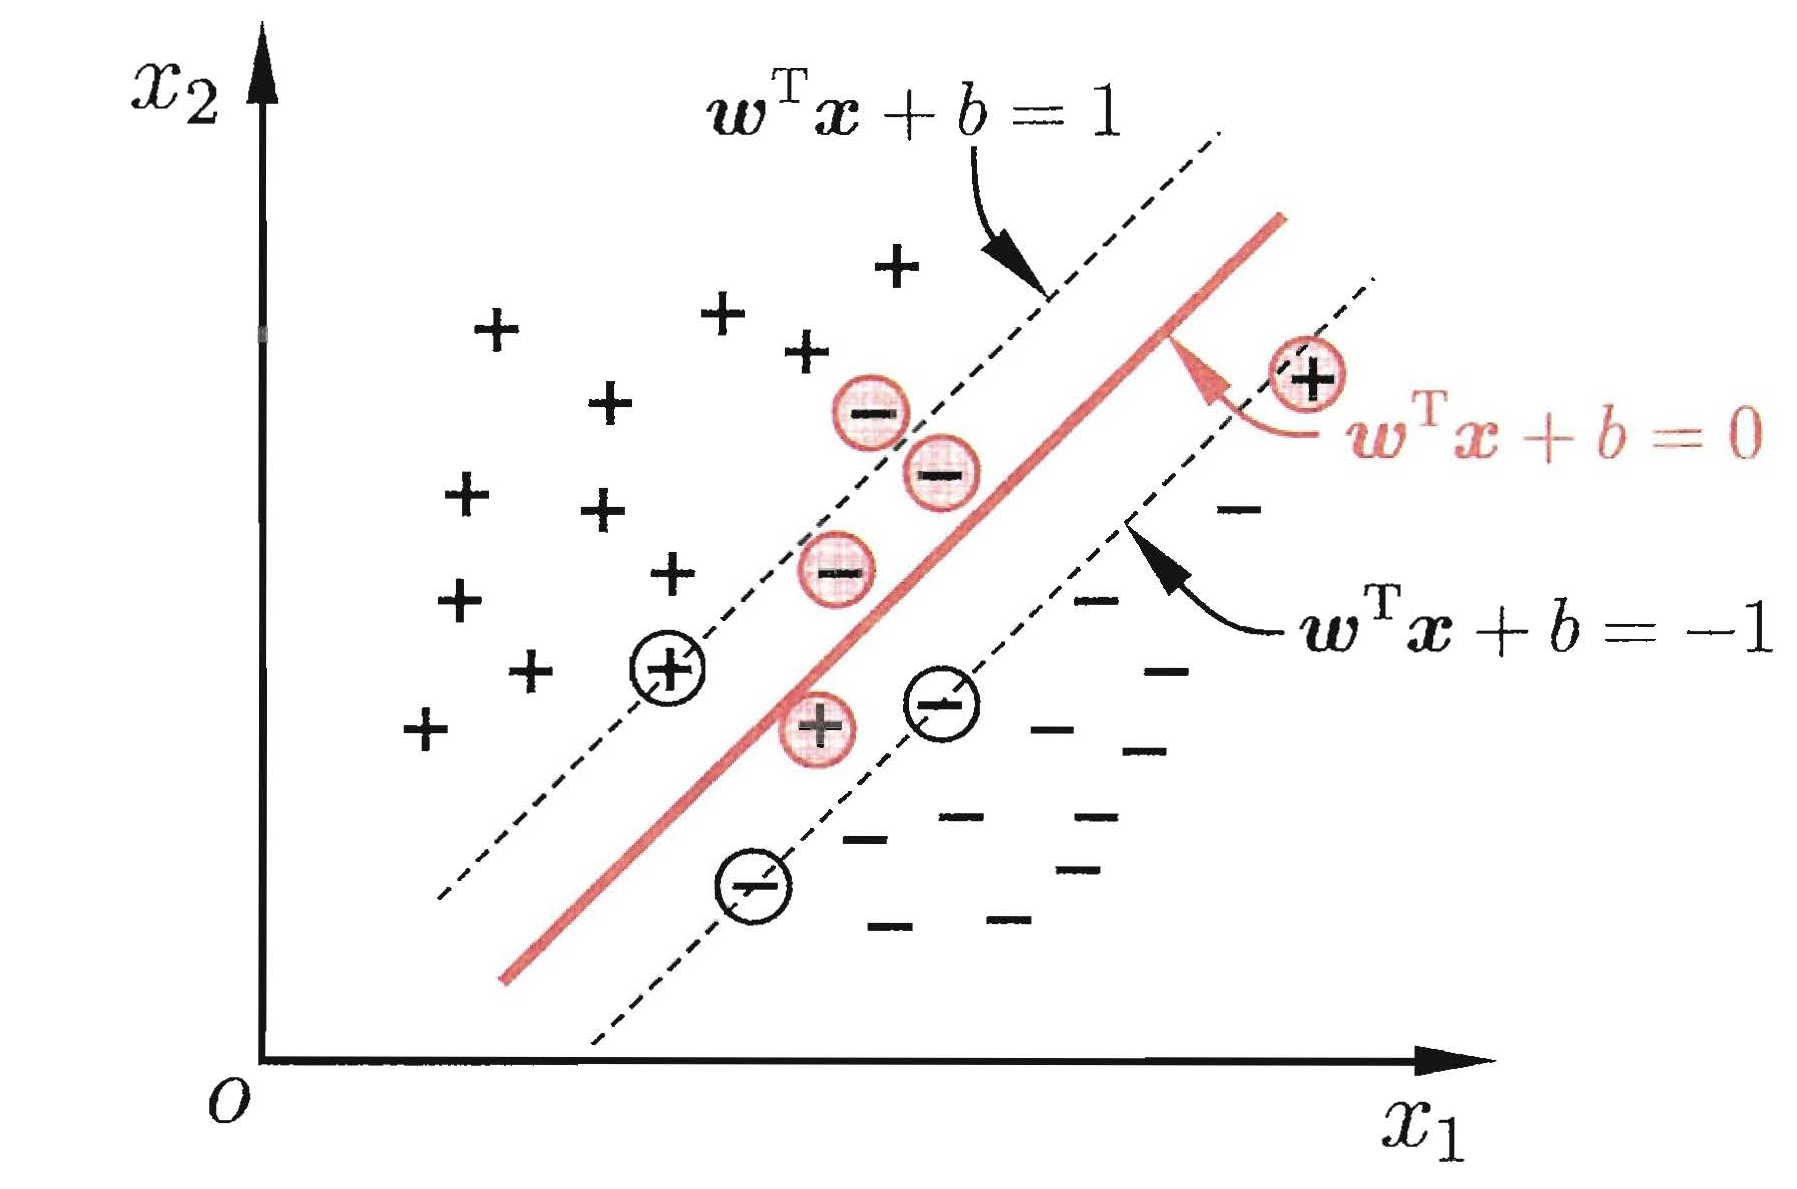
\includegraphics[height=5.5cm]{../image/软间隔.png}
		\caption{软间隔示意图,红色圈出了一些不满足约束的样本。}
		\label{软间隔图}
	\end{figure}
	
	以线性SVM为例,其形式要求所有样本都划分正确,即 $y_{i}\left(\boldsymbol{w}^{\mathrm{T}} \boldsymbol{x}_{i}+b\right) \geqslant 1$,软间隔允许某些样本不满足这一约束。
	
	当然,在最大化间隔的同时,不满足约束的样本应尽可能少。于是,优化目标可
	写为
	
	\begin{equation}
		\min _{\boldsymbol{w}, b} \frac{1}{2}\|\boldsymbol{w}\|^{2}+C \sum_{i=1}^{m} \ell_{0 / 1}\left(y_{i}\left(\boldsymbol{w}^{\mathrm{T}} \boldsymbol{x}_{i}+b\right)-1\right)
		\label{软间隔优化目标}
	\end{equation}
	
	其中 $C>0$ 是一个常数,$\ell_{0/1}$ 是“0/1损失函数”。$\ell_{0/1}$ 非凸、非连续,我们不妨使用hinge损失代替:
	
	\begin{equation}
		\ell_{\text{hinge}}(z)=\max(0,1-z)
	\end{equation}
	
	则式\eqref{软间隔优化目标}可写成
	
	\begin{equation}
		\min _{\boldsymbol{w}, b} \frac{1}{2}\|\boldsymbol{w}\|^{2}+C \sum_{i=1}^{m} \max \left(0,1-y_{i}\left(\boldsymbol{w}^{\mathbf{T}} \boldsymbol{x}_{i}+b\right)\right)
		\label{软间隔用hinge}
	\end{equation}
	
	引入“松弛变量”$\xi_i\geqslant 0$,可将式\eqref{软间隔用hinge}重写为
	
	\begin{equation}
		\begin{aligned}
			\min _{w, b, \xi_{i}}\quad&\frac{1}{2}\|w\|^{2}+C \sum_{i=1}^{m} \xi_{i}\\
			\text{s.t.}\quad&y_i\left(\boldsymbol{w}^{\mathrm{T}}\boldsymbol{x}_i+b\right)\geqslant 1-\xi_i\\
			&\xi_{i}\geqslant0,\quad i=1,2,\cdots,m
		\end{aligned}
		\label{软间隔SVM}
	\end{equation}
	
	这就是常用的软间隔SVM。
	
	式\eqref{软间隔SVM}与式\eqref{主问题}类似,仍是一个二次规划问题;于是,类似式\eqref{拉格朗日函数},通过拉格朗日乘子法可得到式\eqref{软间隔SVM}的拉格朗日函数
	
	\begin{equation}
		L(\boldsymbol{w},b,\boldsymbol{\alpha},\boldsymbol{\xi},\boldsymbol{\mu})=\frac{1}{2}\|\boldsymbol{w}\|^2+C\sum_{i=1}^m\xi_i+\sum_{i=1}^m\alpha_i[1-\xi_i-y_i(\boldsymbol{w}^{\mathrm{T}}\boldsymbol{x}_i+b)]-\sum_{i=1}^m\mu_i\xi_i
		\label{软间隔拉格朗日函数}
	\end{equation}
	
	其中 $\alpha_i\geqslant0$,$\mu_i\geqslant0$ 是拉格朗日因子。
	
	令 $L(\boldsymbol{w},b,\boldsymbol{\alpha},\boldsymbol{\xi},\boldsymbol{\mu})$ 对 $\boldsymbol{w},b,\xi_i$ 的偏导为零可得
	
	\begin{equation}
		\boldsymbol{w}=\sum_{i=1}^m\alpha_iy_i\boldsymbol{x}_i
		\label{软间隔偏导1}
	\end{equation}
	
	\begin{equation}
		\sum_{i=1}^m\alpha_iy_i=0
		\label{软间隔偏导2}
	\end{equation}
	
	\begin{equation}
		C=\alpha_i+\mu_i
		\label{软间隔偏导3}
	\end{equation}
	
	将式\eqref{软间隔偏导1}-\eqref{软间隔偏导3}代入式\eqref{软间隔拉格朗日函数}即可得到式\eqref{软间隔SVM}的对偶问题
	
	\begin{equation}
		\begin{aligned}
			\max _{\boldsymbol{\alpha}} & \sum_{i=1}^{m} \alpha_{i}-\frac{1}{2} \sum_{i=1}^{m} \sum_{j=1}^{m} \alpha_{i} \alpha_{j} y_{i} y_{j} \boldsymbol{x}_{i}^\mathrm{T}\boldsymbol{x}_{j} \\
			\text { s.t. } & \sum_{i=1}^{m} \alpha_{i} y_{i}=0, \\
			& 0\leqslant\alpha_{i} \leqslant C, \quad i=1,2, \ldots, m
		\end{aligned}
	\end{equation}

	在线性的软间隔SVM的基础上,我们引入核函数$\kappa$,对偶问题为
	
	\begin{equation}
		\begin{aligned}
			\max _{\boldsymbol{\alpha}} & \sum_{i=1}^{m} \alpha_{i}-\frac{1}{2} \sum_{i=1}^{m} \sum_{j=1}^{m} \alpha_{i} \alpha_{j} y_{i} y_{j} \kappa\left(\boldsymbol{x}_{i},\boldsymbol{x}_{j} \right)\\
			\text { s.t. } & \sum_{i=1}^{m} \alpha_{i} y_{i}=0, \\
			& 0\leqslant\alpha_{i} \leqslant C, \quad i=1,2, \ldots, m
		\end{aligned}
		\label{核函数软间隔SVM}
	\end{equation}

	类似式\eqref{KKT},软间隔SVM的KKT条件为
	
	\begin{equation}
		\left\{\begin{array}{l}
			\alpha_{i} \geqslant 0,\quad \mu_i\geqslant 0 \\
			y_{i} f\left(\boldsymbol{x}_{i}\right)-1+\xi_i \geqslant 0 \\
			\alpha_{i}\left(y_{i} f\left(\boldsymbol{x}_{i}\right)-1+\xi_i\right)=0\\
			\xi_i\geqslant 0,\quad\mu_i\xi_{i}=0
		\end{array}\right.
		\label{软间隔KKT}
	\end{equation}

	\section{算法设计思路}
	
	\subsection{对偶问题转化}
	
	将式\eqref{核函数软间隔SVM}表示的对偶问题转化为凸优化问题
	
	\begin{equation}
		\begin{aligned}
			\min _{\boldsymbol{\alpha}}\  & \frac{1}{2} \sum_{i=1}^{m} \sum_{j=1}^{m} \alpha_{i} \alpha_{j} y_{i} y_{j} \kappa\left(\boldsymbol{x}_{i},\boldsymbol{x}_{j} \right)-\sum_{i=1}^{m} \alpha_{i}\\
			\text { s.t. } & \sum_{i=1}^{m} \alpha_{i} y_{i}=0, \\
			& 0\leqslant\alpha_{i} \leqslant C, \quad i=1,2, \ldots, m
		\end{aligned}
		\label{凸优化}
	\end{equation}

	根据式\eqref{软间隔KKT}表示的KKT条件和式\eqref{软间隔偏导3}表示的约束条件
	
	\begin{equation}
		\begin{aligned}
			\alpha_i=0\Rightarrow&\ y_if(\boldsymbol{x}_i)-1\geqslant 0\\
			0<\alpha_i<C\Rightarrow&\ y_if(\boldsymbol{x}_i)-1= 0\\
			\alpha_i=C\Rightarrow&\ y_if(\boldsymbol{x}_i)-1\leqslant 0
		\end{aligned}
	\end{equation}
	
	考虑到计算机运算时的误差,我们引入计算误差项 $\varepsilon\geqslant 0$,并记 $E_i=f(\boldsymbol{x}_i)-y_i$,得到
	
	\begin{equation}
		\begin{aligned}
			\alpha_i=0\Rightarrow&\ y_iE_i\geqslant -\varepsilon\\
			0<\alpha_i<C\Rightarrow&\ \left|y_iE_i\right|< \varepsilon\\
			\alpha_i=C\Rightarrow&\ y_iE_i\leqslant \varepsilon
		\end{aligned}
	\end{equation}

	进一步归纳,得到 $\alpha_i$ 的约束条件
	
	\begin{equation}
		\begin{aligned}
			\alpha_i>0\Rightarrow&\ y_iE_i\leqslant\varepsilon\\
			\alpha_i<C\Rightarrow&\ y_iE_i\geqslant-\varepsilon
		\end{aligned}
		\label{alpha约束}
	\end{equation}

	\subsection{SMO算法}
	\subsubsection{基本思想}
	SMO的基本思路是先固定 $\alpha_i$ 之外的所有参数,然后求 $\alpha_i$ 上的极值。由于存在约束 $\sum\limits_{i=1}^m\alpha_iy_i=0$,若固定 $\alpha_i$ 之外的其它变量,则 $\alpha_i$ 可由其它变量导出。于是,SMO算法每次选择两个变量 $\alpha_i$ 和 $\alpha_j$,并固定其它参数。这样,在参数初始化后,SMO不断执行如下步骤直至收敛:
	
	\begin{itemize}
		\item 选取一对需要更新的 $\alpha_i$ 和 $\alpha_j$;
		\item 固定 $\alpha_i$ 和 $\alpha_j$ 以外的参数,求解式\eqref{凸优化}获得更新后的 $\alpha_i$ 和 $\alpha_j$。
	\end{itemize}


	\subsubsection{单变量无约束迭代}
	
	下面来推导更新 $\alpha_i$ 和 $\alpha_j$ 的迭代式。由于 $\boldsymbol{\alpha}$ 中所有维度都是等价的,我们不妨简化问题,选取 $\alpha_1$ 和 $\alpha_2$,推导更新$\alpha_i$ 和 $\alpha_j$ 的迭代式。
	
	令
	
	\begin{equation}
		\Psi(\boldsymbol{\alpha})=\frac{1}{2} \sum_{i=1}^{m} \sum_{j=1}^{m} \alpha_{i} \alpha_{j} y_{i} y_{j} \kappa\left(\boldsymbol{x}_{i},\boldsymbol{x}_{j} \right)-\sum_{i=1}^{m} \alpha_{i}
		\label{求的函数}
	\end{equation}

	我们选取 $\alpha_1$ 和 $\alpha_2$,固定 $\boldsymbol{\alpha}$ 中其它维度,省略 $\Psi(\boldsymbol{\alpha})$ 中的常数项,得到
	
	\begin{equation}
		\begin{aligned}
			\Psi(\alpha_1,\alpha_2)=&\frac{1}{2}\alpha_{1}^2\kappa(\boldsymbol{x}_1,\boldsymbol{x}_1)+\frac{1}{2}\alpha_{2}^2\kappa(\boldsymbol{x}_2,\boldsymbol{x}_2)\\
			&+y_1y_2\alpha_{1}\alpha_{2}\kappa(\boldsymbol{x}_1,\boldsymbol{x}_2)+\nu_1y_1\alpha_{1}+\nu_2y_2\alpha_{2}-\alpha_{1}-\alpha_{2}
		\end{aligned}
	\end{equation}

	其中
	
	\begin{equation}
		\begin{aligned}
			\nu_i&=\sum_{j=3}^m \alpha_{j}y_j\kappa(\boldsymbol{x}_i,\boldsymbol{x}_j)\\
			&=f(\boldsymbol{x}_i)-y_1\alpha_{1}\kappa(\boldsymbol{x}_i,\boldsymbol{x}_1)-y_2\alpha_{2}\kappa(\boldsymbol{x}_i,\boldsymbol{x}_2)-b,\quad i=1,2
			\label{nu}
		\end{aligned}
	\end{equation}
	
	根据约束条件式\eqref{软间隔偏导2},有
	
	\begin{equation}
		\alpha_1y_1+\alpha_{2}y_2=-\sum_{i=3}^m\alpha_{i}y_i=\zeta
		\label{双约束}
	\end{equation}
 
	其中 $\zeta$ 为常数。针对 $\alpha_{1}$ 和 $\alpha_{2}$,假设更新之前为 $\alpha_{1}^\text{old}$ 和 $\alpha_{2}^\text{old}$,更新之后为 $\alpha_{1}^\text{new}$ 和 $\alpha_{2}^\text{new}$;由于$\boldsymbol{\alpha}$ 中其余维度固定,因此必须满足
	
	\begin{equation}
		\alpha_{1}^\text{old}y_i+\alpha_{2}^\text{old}=\alpha_{2}^\text{new}y_1+\alpha_{2}^\text{new}y_2=\zeta
		\label{更新约束}
	\end{equation}
	
	两个变量不好同时求解,可以先求 $\alpha_{2}^\text{new}$,然后根据式\eqref{更新约束}表示$\alpha_{1}^\text{new}$。
	
	由式\eqref{双约束}得
	
	\begin{equation}
		\alpha_{1}=(\zeta-\alpha_2y_2)y_1
		\label{12关系}
	\end{equation}

	将式\eqref{12关系}代入式\eqref{求的函数},得
	
	\begin{equation}
		\begin{aligned}
			\Psi(\alpha_{2})=&\frac{1}{2}(\zeta-\alpha_{2}y_2)^2\kappa(\boldsymbol{x}_1,\boldsymbol{x}_1)+\frac{1}{2}\alpha_{2}^2\kappa(\boldsymbol{x}_2,\boldsymbol{x}_2)+\alpha_{2}y_2(\zeta-\alpha_{2}y_2)\kappa(\boldsymbol{x}_1,\boldsymbol{x}_2)\\
			&+\nu_1(\zeta-\alpha_{2}y_2)+\nu_2y_2\alpha_{2}-(\zeta-\alpha_{2}y_2)y_1-\alpha_{2}
		\end{aligned}
	\end{equation}
	
	令 $\frac{\mathrm{d}\Psi(\alpha_{2})}{\mathrm{d}\alpha_{2}}=0$,得
	
	\begin{equation}
		\alpha_{2}=\frac{y_2[y_2-y_1+v_1-v_2+\zeta(\kappa(\boldsymbol{x}_1,\boldsymbol{x}_1)-\kappa(\boldsymbol{x}_1,\boldsymbol{x}_2))]}{\kappa(\boldsymbol{x}_1,\boldsymbol{x}_1)+\kappa(\boldsymbol{x}_2,\boldsymbol{x}_2)-2\kappa(\boldsymbol{x}_1,\boldsymbol{x}_2)}
		\label{alpha2原始}
	\end{equation}

	将式\eqref{nu}代入式\eqref{alpha2原始},再结合式\eqref{双约束},得未修剪的 $\alpha_{2}^\text{new}$ 为
	
	\begin{equation}
		\alpha_{2}^{\text{unclipped}}=\alpha_{2}^\text{old}+\frac{y_2(E_1-E_2)}{\kappa(\boldsymbol{x}_1,\boldsymbol{x}_1)+\kappa(\boldsymbol{x}_2,\boldsymbol{x}_2)-2\kappa(\boldsymbol{x}_1,\boldsymbol{x}_2)}
		\label{未修剪}
	\end{equation}

	\subsubsection{修剪 $\alpha_{2}^{\operatorname{unclipped}}$}
	
	$\alpha_{i}$ 必须满足不等式约束
	
	\begin{equation}
		0\leqslant\alpha_{i}\leqslant C
	\end{equation}

	式\eqref{未修剪}未考虑到不等式约束,是未修剪的值。下面考虑不等式约束,由式\eqref{更新约束},有
	
	\begin{equation}
		\alpha_{1}^\text{new}=\alpha_{1}^\text{old}+y_1y_2(\alpha_{2}^\text{old}-\alpha_{2}^\text{new})
		\label{alpha1迭代}
	\end{equation}

	当 $y_1=y_2$,由\eqref{alpha1迭代}有
	
	\begin{equation}
		\alpha_{1}^\text{new}=\alpha_{1}^\text{old}+\alpha_{2}^\text{old}-\alpha_{2}^\text{new}
	\end{equation}

	故
	
	\begin{equation}
		0 \leqslant \alpha_{1}^\text{new} \leqslant C \Leftrightarrow \alpha_{1}^{\text {old }}+\alpha_{2}^{\text {old }}-C \leqslant \alpha_{2}^\text{new} \leqslant \alpha_{1}^{\text {old }}+\alpha_{2}^{\text {old }}
	\end{equation}

	又 $0\leqslant \alpha_{i}\leqslant C$,所以
	
	\begin{equation}
		\max\left(0,\alpha_{1}^{\text {old }}+\alpha_{2}^{\text {old }}-C) \leqslant \alpha_{2}^\text{new}\leqslant\min(C,\alpha_{1}^{\text {old }}+\alpha_{2}^{\text {old }}\right)
	\end{equation}

	同理,当 $y_1\neq y_2$ 时
	
	\begin{equation}
		 \max\left(0,\alpha_{2}^{\text {old }}-\alpha_{1}^{\text {old }}\right)\leqslant \alpha_{2}^\text{new} \leqslant \min\left(C,\alpha_{2}^{\text {old }}-\alpha_{1}^{\text {old }}+C\right)
	\end{equation}

	设 $[L,H]$ 为考虑不等式约束后 $\alpha_2$ 的可行域,整理得到
	
	\begin{equation}
		[L,H]=\left\{\begin{matrix}
			\left[\max\left(0,\alpha_{1}^{\text {old }}+\alpha_{2}^{\text {old }}-C),\min(C,\alpha_{1}^{\text {old }}+\alpha_{2}^{\text {old }}\right)\right],&y_1=y_2\\
			\left[\max\left(0,\alpha_{2}^{\text {old }}-\alpha_{1}^{\text {old }}\right),\min\left(C,\alpha_{2}^{\text {old }}-\alpha_{1}^{\text {old }}+C\right)\right],&y_1\neq y_2\\
		\end{matrix}\right.
		\label{alpha2可行域}
	\end{equation}
	
	对 $\alpha_{2}^\text{unclipped}$ 的修剪方法clip为
	
	\begin{equation}
		\alpha_{2}^\text{new}=\operatorname{clip}\left(\alpha_{2}^\text{unclipped}\right) =\left\{\begin{matrix}
			L,&\alpha_2^\text{unclipped}<L \\
			\alpha_2^\text{unclipped},&L\leqslant \alpha_2^\text{unclipped}\leqslant H\\
			H,&\alpha_2^\text{unclipped}>H
		\end{matrix}\right.
		\label{迭代式}
	\end{equation}

	\subsubsection{计算 $\alpha_{1}^{\operatorname{new}}$}
	
	由于式\eqref{alpha2可行域}是从式\eqref{alpha1迭代} 开始,根据不等式约束 $0\leqslant\alpha_{i}\leqslant C$得到,故由 式\eqref{alpha1迭代}得到的 $\alpha_{1}^\text{new}$ 必然满足不等式约束,$\alpha_{1}$ 的迭代式就为式\eqref{alpha1迭代}。
	
	\subsubsection{计算 $b^{\text{new}}$}
	
	若 $0<\alpha_{1}^\text{new}<C$,由式\eqref{fx},有
	
	\begin{equation}
		\begin{aligned}
			b^\text{new}=b_1^\text{new}=&\ y_1-\sum_{i=3}^m\alpha_{i}y_i\kappa(\boldsymbol{x}_1,\boldsymbol{x}_i)-\alpha_{1}^\text{new}y_1\kappa(\boldsymbol{x}_1,\boldsymbol{x}_1)-\alpha_{2}^\text{new}y_2\\
			=&\ (\alpha_{1}^\text{old}-\alpha_{1}^\text{new})y_1\kappa(\boldsymbol{x}_1,\boldsymbol{x}_1)+(\alpha_{2}^\text{old}-\alpha_{2}^\text{new})y_1\kappa(\boldsymbol{x}_1,\boldsymbol{x}_2)-E_1^\text{old}+b^\text{old}
		\end{aligned}
	\end{equation}

	同理,若$0<\alpha_{2}^\text{new}<C$
	
	\begin{equation}
		b^\text{new}=b_2^\text{new}=(\alpha_{1}^\text{old}-\alpha_{1}^\text{new})y_1\kappa(\boldsymbol{x}_1,\boldsymbol{x}_2)+(\alpha_{2}^\text{old}-\alpha_{2}^\text{new})y_1\kappa(\boldsymbol{x}_2,\boldsymbol{x}_2)-E_2^\text{old}+b^\text{old}
	\end{equation}

	若同时满足 $0<\alpha_{1}^\text{new}<C$ 和 $0<\alpha_{2}^\text{new}<C$,则显然有 $b^\text{new}=b_1^\text{new}=b_2^\text{new}$;若 $\alpha_{1}^\text{new},\alpha_{2}^\text{new}\in\{0,C\}$ 且 $L\neq H$,则 $b_1^\text{new},b_2^\text{new}$ 之间的值都能使两个样本满足KKT条件,取 $b^\text{new}=\frac{b_1^\text{new}+b_2^\text{new}}{2}$;若 $\alpha_{1}^\text{new},\alpha_{2}^\text{new}\in\{0,C\}$ 且 $L= H$,则不更新 $b$。
	
	\subsubsection{启发式选择}
	
	根据前面的推导,每一步选择两个维度 $\alpha_{i}$ 和 $\alpha_{j}$ 进行优化
	
	\begin{equation}
		\begin{aligned}
			\alpha_{i}^\text{new}=&\alpha_{i}^\text{old}+y_1y_2(\alpha_{j}^\text{old}-\alpha_{j}^\text{new})\\
			\alpha_{j}^\text{new}=&\operatorname{clip}\left(\alpha_{j}^\text{old}+\frac{y_j(E_i-E_j)}{\kappa(\boldsymbol{x}_i,\boldsymbol{x}_i)+\kappa(\boldsymbol{x}_j,\boldsymbol{x}_j)-2\kappa(\boldsymbol{x}_i,\boldsymbol{x}_j)}\right)
		\end{aligned}
	\end{equation}
	
	注意到只需选取的 $\alpha_{i}$ 和 $\alpha_{j}$ 中有一个不满足式\eqref{alpha约束}的约束,目标函数就会在迭代后减小。所以SMO算法先选取违背式\eqref{alpha约束}的维度,得到 $\alpha_{i}$。选择 $\alpha_{j}$ 的启发规则是选择样本 $\kappa(\boldsymbol{x}_j,y_j)$ 来使得优化的步长最大化,也就是使式\eqref{迭代式}中$\frac{y_j(E_j-E_j)}{\kappa(\boldsymbol{x}_i,\boldsymbol{x}_i)+\kappa(\boldsymbol{x}_j,\boldsymbol{x}_j)-2\kappa(\boldsymbol{x}_i,\boldsymbol{x}_j)}$最大化。由于计算核函数比较耗时间,所以SMO使用简单的近似,用 $|E_i-E_j|$ 来近似步长;也就是说,选择样本 $(\boldsymbol{x}_j,y_j)$ 使 $|E_i-E_j|$ 最大,$\alpha_{j}$ 的更新步长就能尽可能大。
	
	\subsection{算法流程总结}
	
	经过上面的讨论,算法流程如图\ref{算法流程}所示。
	
	\begin{figure}[!htb]
		\centering
		\scriptsize  
		% 流程图定义基本形状
		\tikzstyle{startstop} = [rectangle, rounded corners, minimum width = 2cm, minimum height=0.5cm,text centered, draw = black]
		\tikzstyle{io} = [trapezium, trapezium left angle=80, trapezium right angle=100, minimum width=1cm, minimum height=0.6cm, text centered, draw=black]
		\tikzstyle{process} = [rectangle, minimum width=3cm, minimum height=0.6cm, text centered, draw=black]
		\tikzstyle{decision} = [diamond, aspect = 3, text centered, draw=black]
		\tikzstyle{point}=[coordinate,on grid] 
		% 箭头形式
		\tikzstyle{arrow} = [->,>=stealth]
		\begin{tikzpicture}
			\node[startstop](start){ 开始};
			\node[io,right=of start](define){ 输入数据集 $D=\{(\boldsymbol{x}_i,y_i)\}_{i=1}^m$};
			\node[process,right=of define](init){ 初始化参数 $\boldsymbol{\alpha}=\boldsymbol{O},b=0$};
			\node[decision,below=of init](decision){ 迭代次数 < $\text{MAX\_ITER}$};
			\node[process,below=of decision](choose){启发式选择 $\alpha_{i},\alpha_{j}$};
			\node[io,left=of decision](output){输出$\boldsymbol{\alpha},b$};
			\node[process,below=of choose](update){按更新 $\alpha_{i},\alpha_{j},b$};
			\node[point,right of=update,node distance=2.6cm](point1){};
			\node[startstop,left=of output](stop){结束};
			\draw[arrow](start)--(define);
			\draw[arrow](define)--(init);
			\draw[arrow](init)--(decision);
			\draw[arrow](decision)--node[right]{是}(choose);
			\draw[arrow] (decision)-- node[above]{否}(output);
			\draw[arrow](choose)--(update);
			\draw[-](update)--(point1);
			\draw[arrow](point1)|-(decision);
			\draw[arrow](output)--(stop);
		\end{tikzpicture}
		\caption{算法流程}
		\label{算法流程}
	\end{figure}

	\section{核心代码分析}
	\subsection{数据定义}
	代码中定义最大迭代次数,用矩阵$\mathbf{X}$表示西瓜数据集$3.0\alpha$的数据部分,每个样本有密度、含糖率两个维度,用向量 $y$ 表示每个西瓜的真实标记。初始化 $\boldsymbol{\alpha}=\boldsymbol{O}$,$b=0$。定义常数 $C=1$,$\varepsilon=0.00001$。
	\lstinputlisting[style=Python]{../code/core/init.txt}
	\subsection{定义核函数 $\kappa$}
	kappa函数提供六种核函数,包括线性核、高斯核、多项式核、拉普拉斯核、Sigmoid核、RBF核,函数默认使用高斯核。
	\lstinputlisting[style=Python]{../code/core/kappa.txt}
	\subsection{修剪操作}
	修剪操作,实际上就是让超过可行域的取值 $a$ 落到可行域的边界上。
	\lstinputlisting[style=Python]{../code/core/clip.txt}
	\subsection{SMO过程}
	按照图\ref{算法流程}的流程,每一次迭代都按照启发式规则选择 $\alpha_{i}$ 和 $\alpha_{j}$:首先选择不满足式\eqref{alpha约束}的$\alpha_{i}$,若都满足约束则随机选择;接着再选择 $\alpha_{\underset{1\leqslant j\leqslant m,j\neq i}{\arg \max }|E_i-E_j|}$,更新 $\alpha_{i}$、$\alpha_{j}$、$b$。\\
	\lstinputlisting[style=Python]{../code/core/smo.txt}
	\subsection{结果预测}
	利用式\eqref{fx}得到 $f(\boldsymbol{x}_i)$。
	\lstinputlisting[style=Python]{../code/core/predict.txt}
	\section{实验结果与分析}
	
	此次实验中用到了表\ref{核函数表}中所列举的核函数,使用不同核函数,对西瓜数据集 $3.0\alpha$ 的分类效果如图\ref{linear}-\ref{laplace}所示。
	
	\begin{figure}[!htb]
		\centering
		\begin{minipage}{0.49\linewidth}
			\centering
			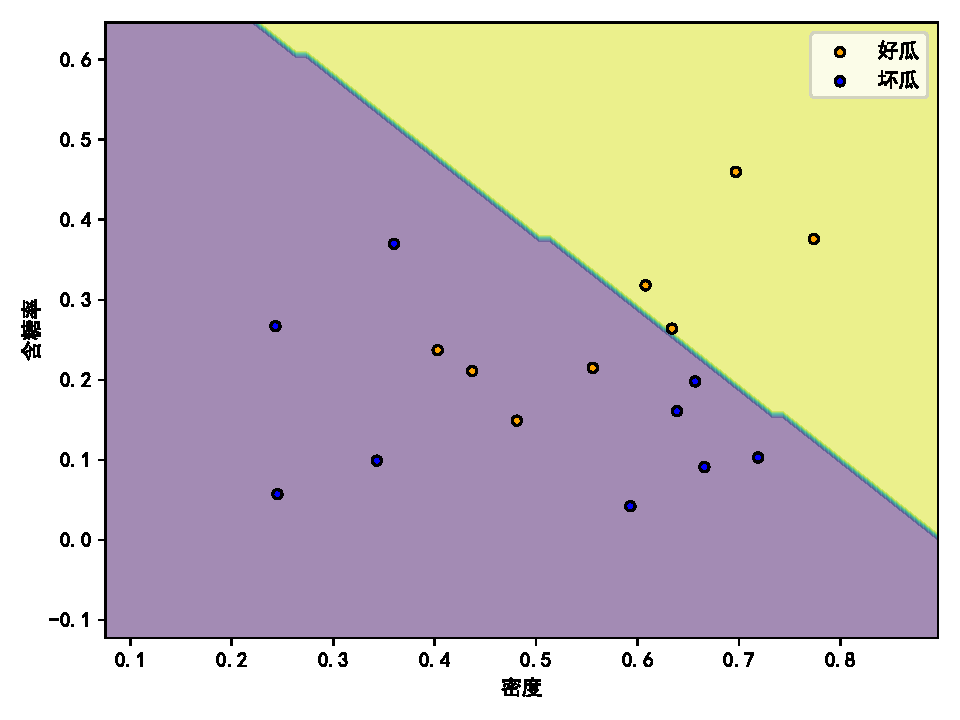
\includegraphics[width=\textwidth]{../image/线性核.pdf}
			\caption{线性核}
			\label{linear}%文中引用该图片代号
		\end{minipage}
		\begin{minipage}{0.49\linewidth}
			\centering
			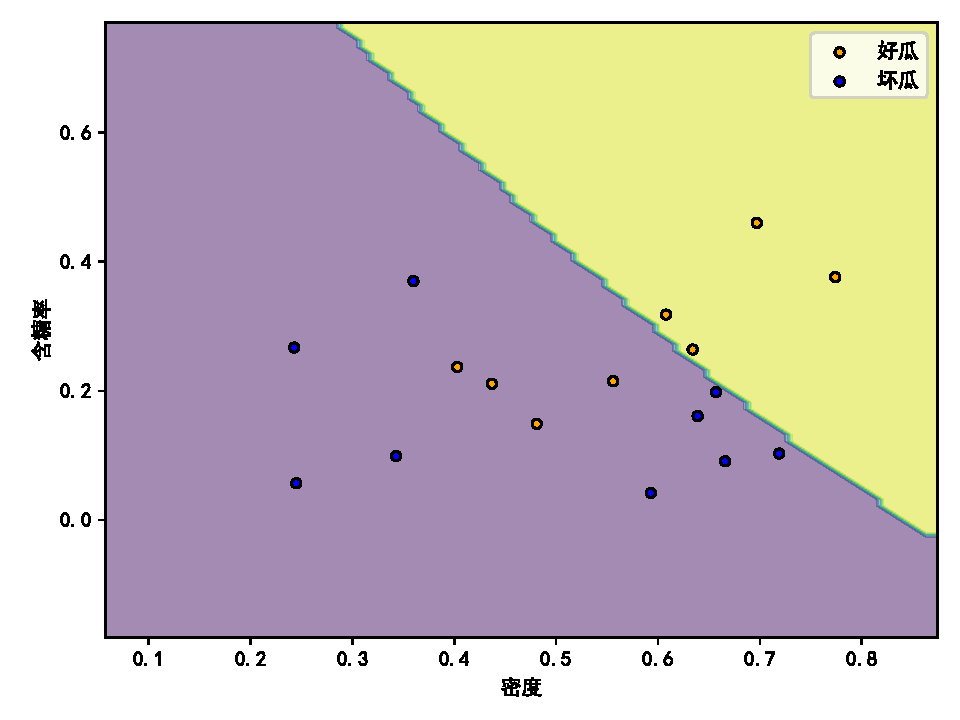
\includegraphics[width=\textwidth]{../image/多项式核.pdf}
			\caption{多项式核}
			\label{poly}%文中引用该图片代号
		\end{minipage}
	
		\begin{minipage}{0.49\linewidth}
			\centering
			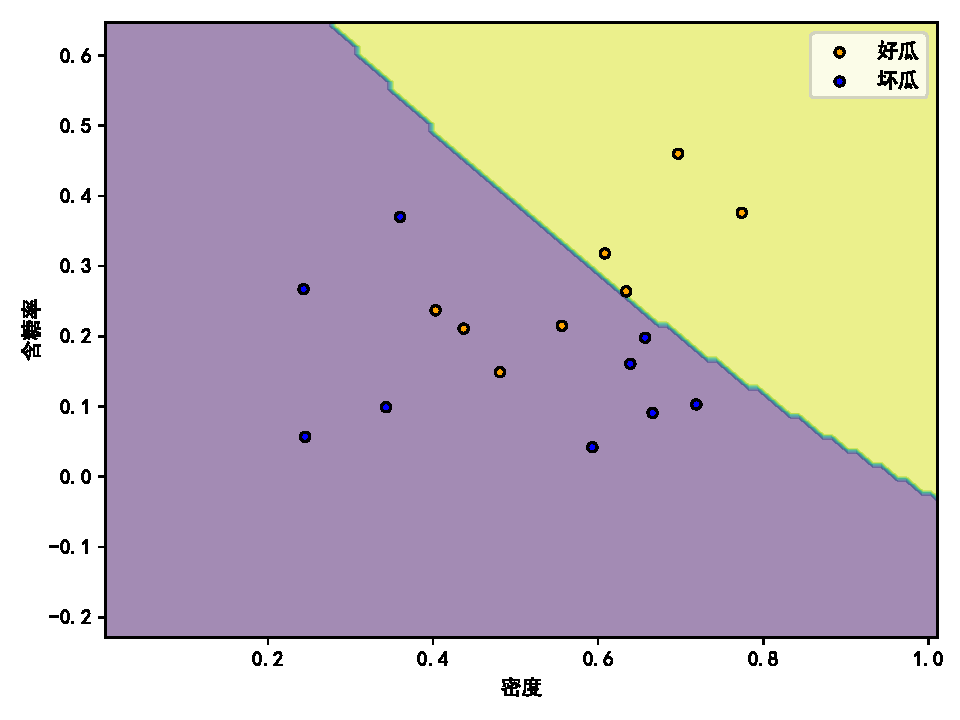
\includegraphics[width=\textwidth]{../image/RBF核.pdf}
			\caption{RBF核}
			\label{rbf}
		\end{minipage}
		\begin{minipage}{0.49\linewidth}
			\centering
			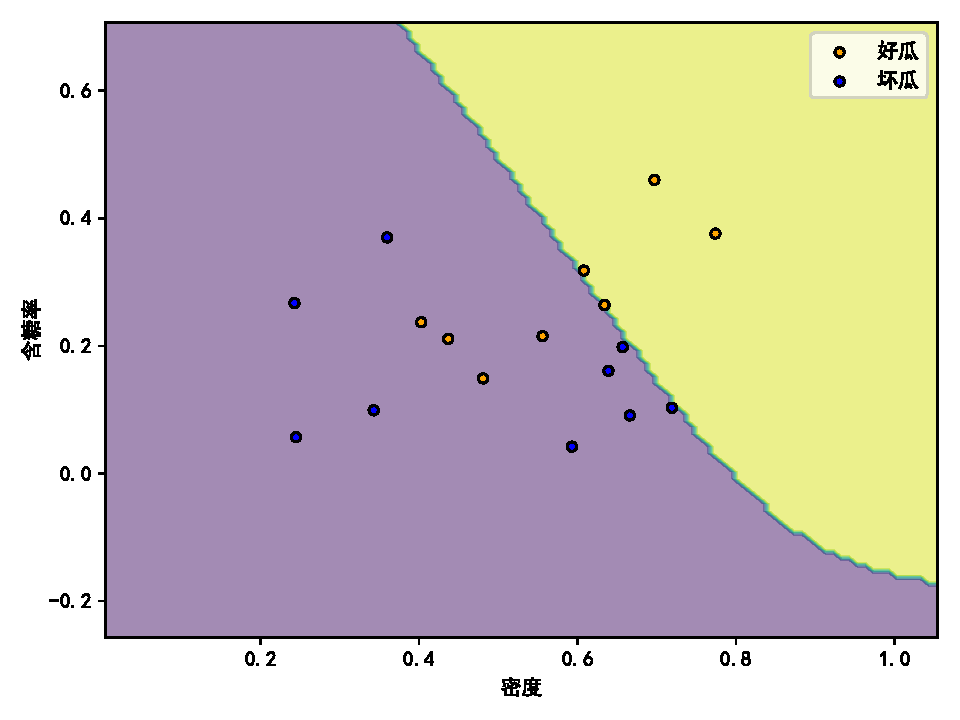
\includegraphics[width=\textwidth]{../image/Sigmoid核.pdf}
			\caption{Sigmoid核}
			\label{sigmoid}
		\end{minipage}
		
		\begin{minipage}{0.49\linewidth}
			\centering
			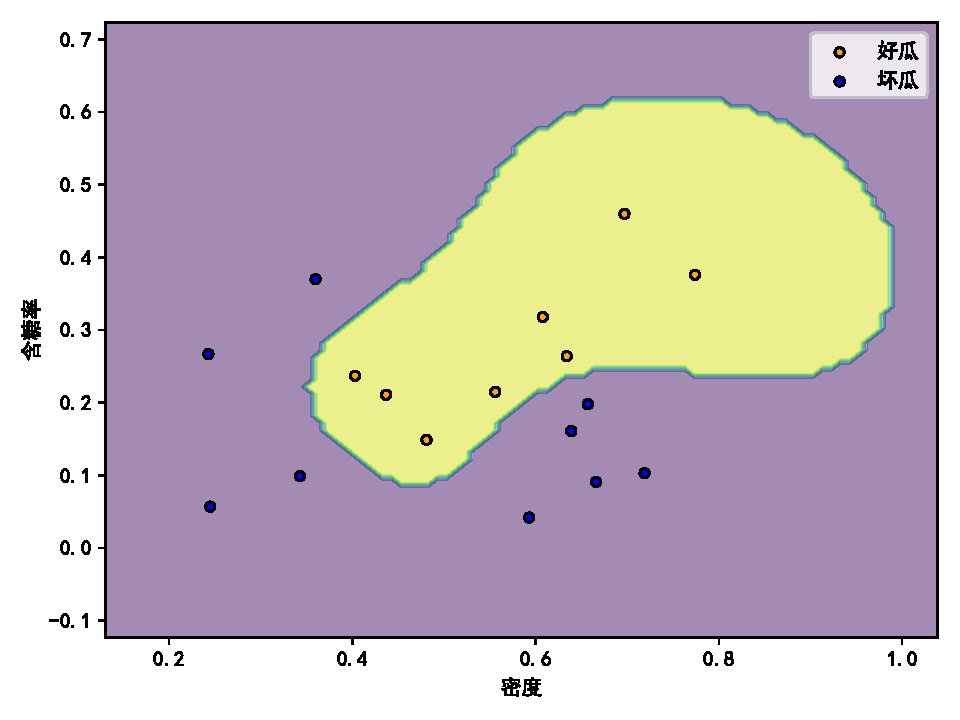
\includegraphics[width=\textwidth]{../image/高斯核.pdf}
			\caption{高斯核}
			\label{gauss}
		\end{minipage}
		\begin{minipage}{0.49\linewidth}
			\centering
			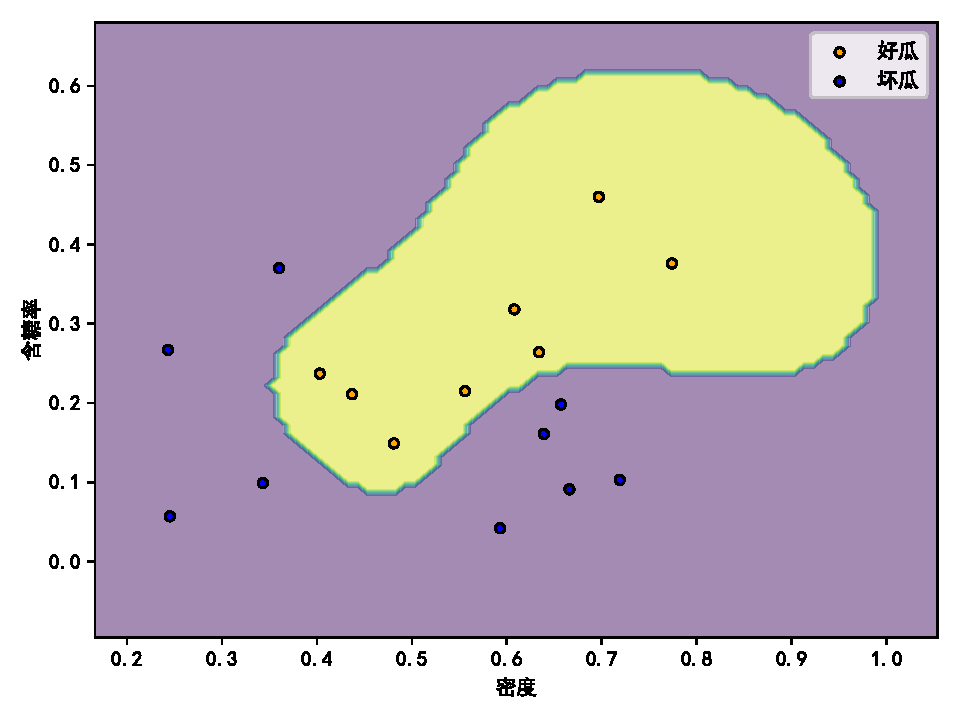
\includegraphics[width=\textwidth]{../image/拉普拉斯核.pdf}
			\caption{拉普拉斯核}
			\label{laplace}
		\end{minipage}
	\end{figure}

	基于在西瓜数据集 $3.0\alpha$ 上的分类效果,我们可以初步得到如下结论:
	
	\begin{itemize}
		\item 线性核、多项式核、RBF核、Sigmoid核的分类效果类似,都没有将好瓜与坏瓜完全区分开来;
		\item 高斯核、拉普拉斯核的分类效果相似,将好瓜与坏瓜完全区分开来。
	\end{itemize}
	
	如表\ref{核函数表}所示,高斯核、拉普拉斯核、RBF核的数学形式相似,因此高斯核、拉普拉斯核的分类效果相似,RBF核分类效果差的原因在于 $\gamma$ 取值的限制。在scikit-learn提供的SVM包中,取消了 $0<\gamma<1$ 这一限制,仅提供RBF核和拉普拉斯核核,并默认 $\gamma=\frac{1}{\text{n\_features}\cdot\text{X.var()}}$,也能取得较好的分类效果。
	
	线性核、多项式核、Sigmoid核表示的函数在二维空间中都是不封闭的曲线,可以看到二维空间中的分类边界就类似这些函数的曲线,仅从西瓜数据集 $3.0\alpha$来看,并不适合作为SVM的核函数。
	
	线性核计算快、可计算得到明确的边界,但是只能解决线性可分问题。多项式核、Sigmoid核可解决非线性问题,多项式核对于大数量级的幂数计算较慢,而Sigmoid核更常用于训练多层感知机神经网络。高斯核、RBF核、拉普拉斯核能将样本映射到无穷维空间,决策边界更为多样,分类效果好,但是难以计算清晰的分类边界。
	
	\section{学习收获}
	
	在这次实验过程中,我从头实现了SVM,并对多个不同核函数的分类效果进行了比较。基于西瓜数据集 $3.0\alpha$ 上的分类效果,得出了不同核函数的优缺点和适用场景。
	
	关于SMO方法、KKT条件等知识,书上提及甚少,我因此查阅了大量资料,自己推导了SMO算法的诸多迭代式。实际上,在SMO过程中,我们还可以动态更新 $E_i$,而不必每一步迭代都重新计算 $E_i$,将来需要在代码中完善这一过程,进而提高训练SVM的速度。
	
	此次实验还留下疑问,即Sigmoid核与多层感知机神经网络之间的联系。
	
	\section{参考资料}
	\begin{itemize}
		\item 《机器学习》6.1,6.2,6.3,6.4;周志华;清华大学出版社
		\item \href{https://scikit-learn.org.cn/view/83.html}{支持向量机(scikit-learn中文社区)}
		\item \href{https://scikit-learn.org.cn/view/781.html}{sklearn.svm.SVC(scikit-learn中文社区)}
		\item \href{https://www.quora.com/Why-does-the-RBF-radial-basis-function-kernel-map-into-infinite-dimensional-space-mentioned-many-times-in-machine-learning-lectures/answer/Arun-Iyer-1}{Why does the RBF (radial basis function) kernel map into infinite dimensional space, mentioned many times in machine learning lectures?}
		\item \href{https://www.bilibili.com/video/BV1Mh411e7VU?p=8}{【吃瓜教程】《机器学习公式详解》(南瓜书)与西瓜书公式推导直播合集 | 第六章-支持向量机}
		\item \href{https://blog.csdn.net/luoshixian099/article/details/51227754}{【机器学习详解】SMO算法剖析}
		\item \href{https://dataaspirant.com/svm-kernels/}{SEVEN MOST POPULAR SVM KERNELS}
		\item \href{https://zhuanlan.zhihu.com/p/53759576}{支持向量机(SVM)| SMO方法篇}
		\item \href{https://zhuanlan.zhihu.com/p/29212107}{机器学习算法实践-SVM中的SMO算法}
		\item \href{https://zhuanlan.zhihu.com/p/65453337}{支持向量机原理详解(五): KKT条件(Part II)}
		\item \href{https://zhuanlan.zhihu.com/p/64580199}{支持向量机原理详解(六): 序列最小最优化(SMO)算法(Part I)}
	\end{itemize}
\end{document} 